\section{Introduction: Lattices}\label{sec:lattice_intro}
    A \textit{lattice} is essentially the set of all integer-coefficient linear combinations 
    of a given set of $n$-length basis vectors, forming a grid-like 
    pattern in $n$-dimensional space.
    More formally, if $\v{b}_1,\cdots,\v{b}_n \in \mathbb{R}^n$ are $n$ linearly independent basis vectors 
    we can define a lattice $\mathcal{L}$ as
\begin{equation*}
    \mathcal{L}(\v{b}_1,\cdots,\v{b}_n) = \left\{\sum_{i=1}^n{x_i\v{b}_i : x_i \in \mathbb{Z}}\right\}
\end{equation*}
\begin{figure}[h!]
    \caption{An example of a 2-dimensional lattice with basis vectors [1]}
    \centering
    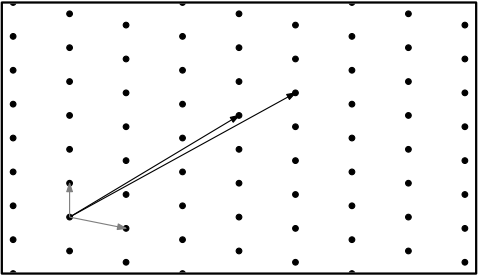
\includegraphics[scale=0.3]{lattice.png}
\end{figure}
We usually represent the basis as a matrix 
\begin{equation*}
    \v{B} = [\v{b_1}, cdots, \v{b_n}] \in \mathbb{R}^{n \times n}
\end{equation*}
so that the lattice generated by $\v{B}$ is
\begin{equation*}
    \mathcal{L}(\v{B}) = \{\v{Bx}: \v{x} \in \mathbb{Z}^n\}.
\end{equation*}
We usually consider \textit{q-ary lattices}, which are lattices whose
member vectors are integers determined component-wise mod $q$ - that
is the are elements of $\mathbb{Z}_q^n$.

Alternatively, if we wish to construct a lattice from a matrix, instead
of using its columns as the basis vectors we can use its rows to 
generate the lattice. This method has the advantage that we can construct
lattice from non-square matrices. Given $\v{A} \in \mathbb{Z}_q^{n \times m}$, define
\begin{equation}
    \Lambda_q(\v{A}) := \{\v{x} \in \mathbb{Z}^m: \v{x} = \v{A}^T\v{s}
        \pmod{q} \text{ for some } \v{s} \in \mathbb{Z}^n
    \}
\end{equation}

Before describing Learning With Errors, we first describe two traditional
lattice problems that can be reduced to it.
First is the Shortest Vector Problem (SVP), formulated as follows:
Given a basis $\v{B}$ and approximation factor $\gamma$, find a vector 
$\v{x}$ such that $||\v{x}|| \leq \gamma||\v{s}||$, where $\v{s}$ is
the shortest nonzero vector in $\mathcal{L}(\v{B})$.

Next is the Shortest Independent Vector Problem (SIVP): Given basis
$\v{B}$ and approximation factor $\gamma$, find $n$ linearly 
independent lattice vectors $\{\v{x}_1, \cdots, \v{x}_n\} \subseteq
\mathcal{L}(\v{B})$ such that $\max_i{||\v{x}_i||} \leq \gamma S$,
where $S = \max_i{||\v{x}_i||}$ for the set of $n$ linearly independent
vectors $\{\v{x}_1,\cdots,\v{x}_n\}$ giving the smallest such quantity $S$ (both problems involve finding approximations to the optimal
solution to the problem).

Existing algorithms to solve these two problems either run in polynomial time but only for exponential approximation factors $\gamma$, or can
approximate the solution to within polynomial factors but can only
achieve exponential run time. Thus [1] conjectures that there is no 
polynomial time classical or quantum algorithm that approximates these
lattice problems to within polynomial factors.
